\section{Степенные законы распределения}

В этой части я расскажу о функциях распределения и о том, почему мы должны обратить на них внимание. Я проделаю это на примере конкретных данных обанкротившейся компании Энрон (Enron Corporation).

Энрон - компания, достигшая большого успеха в области энергетики. Однако компания обанкротилась в 2001 году в результате бухгалтерских махинаций и сокрытия реальных доходов\cite{enron_fall}. Корпус Энрон (Enron corpus) - публичный набор данных с историей почтовых сообщений внутри компании.

\begin{figure}[H]
 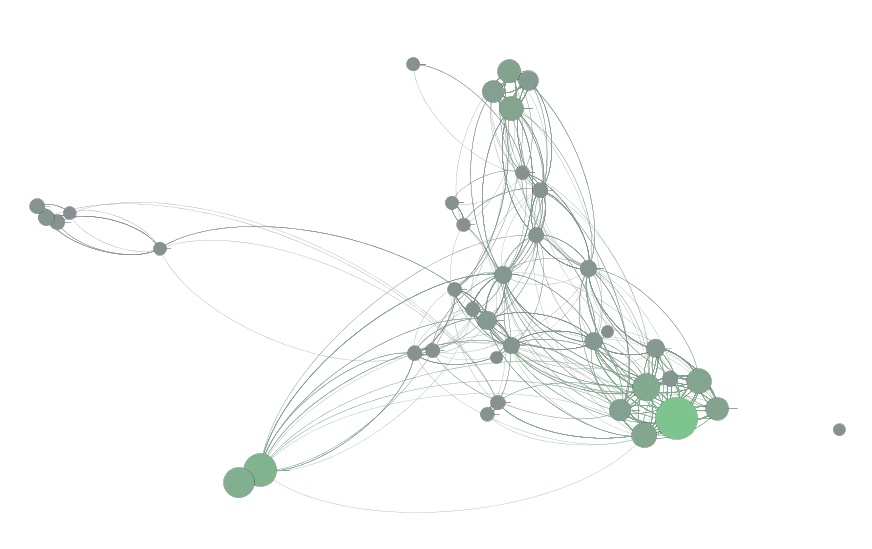
\includegraphics[width=1\linewidth]{recources/enron/enron_social_network_graph}
 \caption{Граф социальных связей для корпуса Энрон. Вершины - сотрудники компании, а ребра - пересылаемые между ними сообщения.}
 \label{fig:enron_social_network_graph}
\end{figure}

С одной стороны этот корпус может представлять большой интерес для анализа, а с другой стороны он достаточно мал (примерно полмиллиона сообщений между 158 сотрудниками\cite{sims_sinitsyn_matrix_structures}). На рис.~\ref{fig:enron_social_network_graph} можно увидеть внешний вид графа пересылаемых сообщений. Крупные вершины в графе соответствуют более активным пользователям почты.

Функции распределения сами по себе уже давно не являются чем-то новым и необычным. Очень много вещей и величин например распределены по нормальному закону. Это происходит из следствия предельной теоремы, которое говорит о том, что если есть множество случайных распределений, то сумма этих распределений будет похожа на нормальное распределение. 

Так распределены, например, рост человека или максимальная скорость автомобилей. Если мы говорим о распределении роста человека, то оно близко к нормальному, имеется ярко выраженный узкий пик и очень быстро затухающие хвосты. 


Конечно же не все величины в природе распределены нормально. Есть множество исключений, это можно показать на примере зависимости количества человек, отправивших определенное количество сообщений, от количества сообщений. В этом случае уже нет пика, функция всегда убывает. Это говорит о том, что случайно выбранный человек с большей вероятностью окажется с небольшим количеством отправленных сообщений и с очень низкой вероятностью с огромным. 

\begin{figure}[H]
 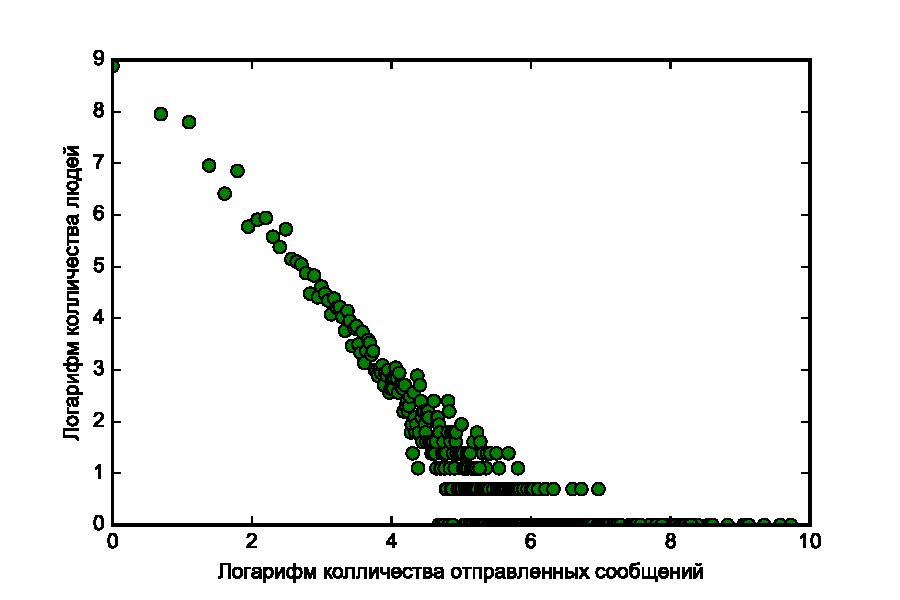
\includegraphics{recources/enron/mailes_by_people_enron}
 \caption{График зависимости количества человек от количества сообщений, которе они отправили в логарифмических координатах. Из графика видно, зависимость имеет ярко выраженную степенную зависимость.}
 \label{fig:enron_mails_by_people}
\end{figure}

Важно отметить, что встречаются сотрудники с очень большим количеством отправленных сообщений, которое больше количества отправленных сообщений большинства других сотрудников на порядки, т.е. у этого распределения есть длинных хвост. И этот хвост затухает не экспоненциально, не быстро. 

Если это распределение построить в логарифмических координатах(Рис.~\ref{fig:enron_mails_by_people}), то оно станет гораздо нагляднее и примет вид близкий к прямой. Такого вида распределения мы и будем называть \textit{степенными распределениями}. 

Это распределение имеет вид \cite{zhukov} $$ p(x) = Cx^{-\alpha} = \frac{C}{x^\alpha} \text{, для } x \ge x_{min} $$ 
Нормировка дает значение константы $C = (\alpha - 1) x_{min}^{\alpha - 1}$.
Таким образом в общем виде степенное распределение имеет вид $$p(x) = \frac{\alpha - 1}{x_{min}} \left( \frac{x}{x_{min}} \right)^{-\alpha}$$

Стоит отметить, что в этом законе распределения участвует две константы: $\alpha$ и $x_{min}$. Таким образом получается, что закон ведет себя немного по разному в зависимости от выбора начально значения. Это обусловлено тем, что нельзя определить закон из нуля.

Если посмотреть на Рис.~\ref{fig:enron_mails_by_people}, то видно, что вост очень размыт. Поскольку $\alpha$ это по сути коэффициент наклона прямой на графике, то удобно ввести т.н. комплементарную кумулятивную функцию распределения (complimentary cumulative distribution function, cCDF).

По определению кумулятивная функция распределения(cumulative distribution function, CDF) это: 
$$ F(x) = Pr(X \le x) = \int_{-\infty}^x p(y)dy = \int_{x_{min}}^x p(y)dy $$
а комплементарная CDF это:
$$ \bar F(x) = 1 - F(x) = P(X > x) = \int_x^\infty p(y)dy $$

Таким образом, если наш закон распределения является степенным, т.е. $p(x) = Cx^{-\alpha}$, то cCDF примет вид:
$$ \bar F(x) = \frac{C}{\alpha - 1} x^{-(\alpha - 1)} = 
\left( \frac{x}{x_{min}} \right)^{-(\alpha - 1)}$$

\begin{figure}[H]
 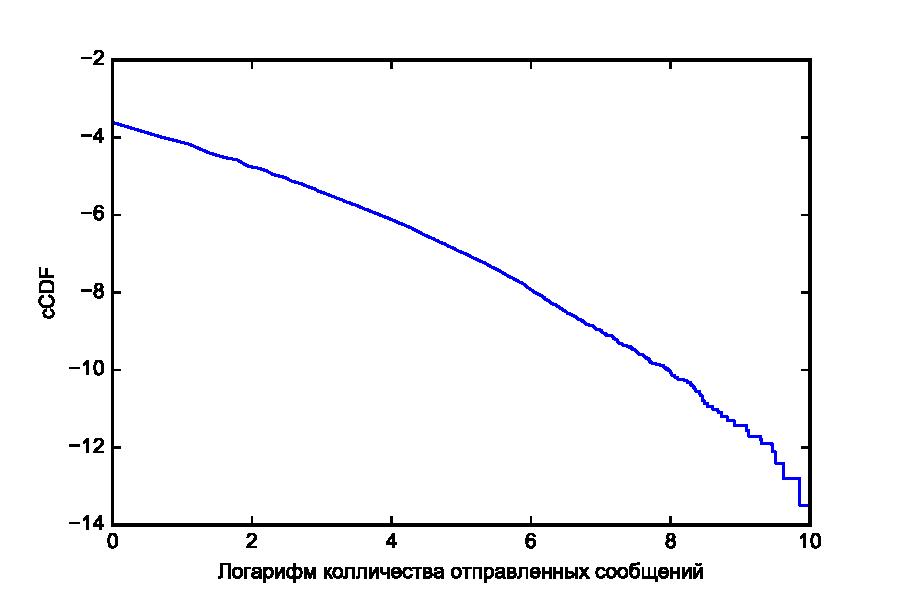
\includegraphics{recources/mailes_by_people_enron_ccdf}
 \caption{Комплиментарная кумулятивная нормированная функция распределения для корпуса Enron в логарифмических координатах.}
 \label{fig:enron_mails_by_people_ccdf}
\end{figure}

На рис.~\ref{fig:enron_mails_by_people_ccdf} изображена комплементарная кумулятивная функция распределения для распределения людей по количеству отправленных писем для корпуса Энрон.



